\chapter{Sparsity, inverse problems and compressed sensing}
\label{chap-sparsity}
\chapteroverview{How can a small number of measurements describe a complicated signal? Sparse representations provide a link between compression and the recovery of incomplete or noisy data. This chapter develops that link, explains the role of convex optimization, and states the assumptions under which compressed sensing gives reliable reconstructions.}

\section{From continuous signals to samples}
\label{sec-sampling}
An acquisition device turns a continuous signal $\tilde f$ into a finite vector $f=(f_q)_{q=1}^Q\in\RR^Q$. For sound, these entries represent measurements at successive times. For a grayscale image, they represent light collected over small sensor regions. An idealized pixel measurement is
\[
 f_q=\int_{c_q}\tilde f(s)\,\d s,
\]
where $c_q$ is the area of the sensor element. Dividing by its area gives an average intensity; exposure time and calibration introduce further scale factors. Color and multichannel signals can be handled by recording several values at each location.

\begin{figure}[htbp]\centering
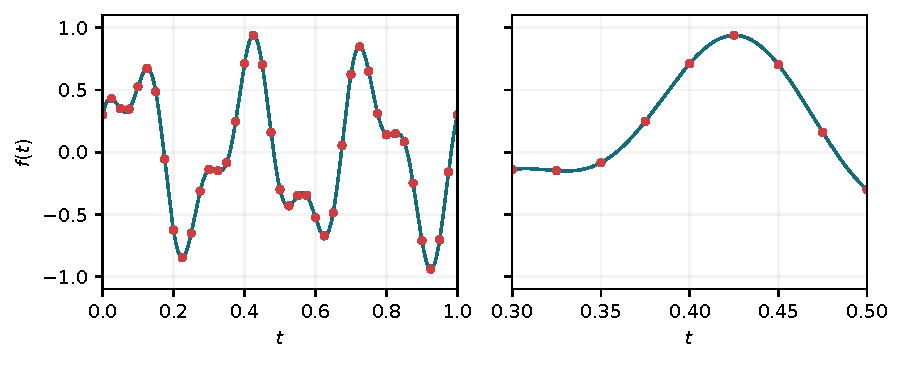
\includegraphics[width=.48\linewidth]{chapter-sampling/discrete-signal.pdf}\hfill
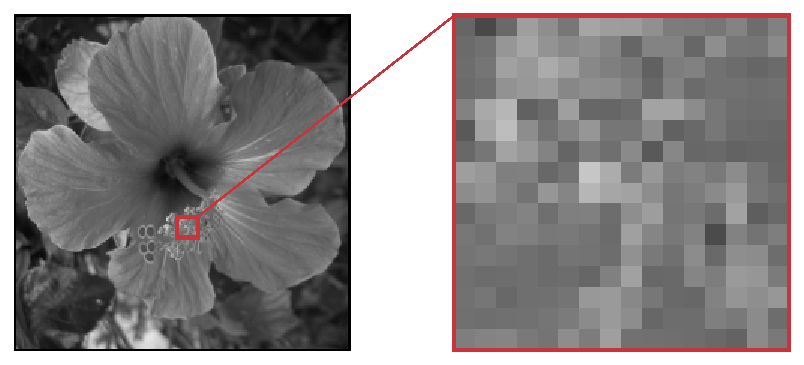
\includegraphics[width=.48\linewidth]{chapter-sampling/discrete-image.pdf}
\caption{Sampling a one-dimensional signal and a two-dimensional image. The dots mark time samples; the red frames identify the image region enlarged on the right.}\label{fig-samples}
\end{figure}

Sampling preserves information only under suitable assumptions. For example, let $\tilde f\in L^2(\RR)$ have Fourier transform supported in $[-B,B]$, with frequency measured in cycles per unit time. If the sampling interval satisfies $0<T<1/(2B)$, the sampling theorem~\cite{shannon1949} gives
\[
 \tilde f(t)=\sum_{k\in\ZZ}\tilde f(kT)\,
 \operatorname{sinc}\!\left(\frac{t}{T}-k\right),
 \qquad \operatorname{sinc}(u)=\begin{cases}\sin(\pi u)/(\pi u),&u\ne0,\\1,&u=0.\end{cases}
\]
For the continuous representative of this band-limited function, the series converges in $L^2$ and uniformly. The theorem uses samples over the entire time axis. A finite recording, quantization, and measurement noise introduce additional errors. Frequencies above the acquisition band must be attenuated before sampling to avoid aliasing; increasing numerical precision afterwards cannot undo aliasing.

This is a different question from lossless coding: sampling concerns the representation of a continuous signal by measurements, whereas coding concerns the binary representation of those measurements. Sparsity provides another useful assumption on the signal, and leads to a different acquisition strategy.

\Needspace{6\baselineskip}
\section{Nonlinear approximation and compression}
\subsection{Sparse representations}
A dictionary $\Psi=(\psi_n)_{n=1}^N$ consists of vectors $\psi_n\in\RR^Q$. We seek an approximation
\[
 f\approx\Psi x=\sum_{n=1}^N x_n\psi_n
\]
using few nonzero coefficients. Sinusoids, local cosine functions, and wavelets are familiar examples of atoms. Transform coding uses such representations to concentrate much of a signal's energy in a small number of coefficients.

Given an integer budget $0\le M\le N$, a best $M$-term approximation solves
\begin{equation}\label{eq-pbm-approx}
 x^\star\in\arg\min_{x\in\RR^N,\;\norm{x}_0\le M}\norm{f-\Psi x}_2^2,
 \qquad \norm{x}_0=\#\{n:x_n\ne0\}.
\end{equation}
Here $\norm{v}_2^2=\sum_n|v_n|^2$. The notation $\norm{x}_0$ is conventional: this count is not a norm, since multiplying a nonzero vector by a nonzero scalar leaves the count unchanged. For a general dictionary, sparse approximation is NP-hard~\cite{Natarajan95}. Exhaustively testing the possible supports is usually prohibitive; this worst-case difficulty does not rule out efficient algorithms for special dictionaries or particular data.

\subsection{The orthonormal case}
Suppose $N=Q$ and $\Psi$ is an orthonormal basis, so that $\langle\psi_n,\psi_m\rangle=\delta_{nm}$. With $a_n=\langle f,\psi_n\rangle$, Parseval's identity gives
\begin{equation}\label{eq-expansion-bon}
 f=\sum_{n=1}^N a_n\psi_n,
 \qquad \norm{f-\Psi x}_2^2=\sum_{n=1}^N|a_n-x_n|^2.
\end{equation}
Once a support is chosen, the best coefficients are the corresponding $a_n$. To minimize the discarded energy, keep the $M$ largest magnitudes. More precisely, choose an ordering $|a_{n_1}|\ge\cdots\ge|a_{n_N}|$. Then
\begin{equation}\label{eq-formule-thresh}
 x_n^\star=\begin{cases}
 a_n,&n\in\{n_1,\ldots,n_M\},\\
 0,&\text{otherwise}.
 \end{cases}
\end{equation}
Ties at the threshold can produce several minimizers. If fewer than $M$ coefficients are nonzero, the approximation uses fewer than $M$ terms.

\begin{figure}[htbp]\centering
\begin{tabular}{@{}c@{\hspace{2mm}}c@{\hspace{2mm}}c@{\hspace{2mm}}c@{}}
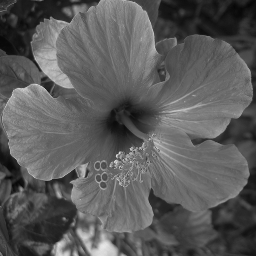
\includegraphics[width=.235\linewidth]{chapter-sampling/original.png}&
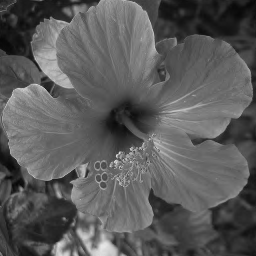
\includegraphics[width=.235\linewidth]{chapter-sampling/approx-4.png}&
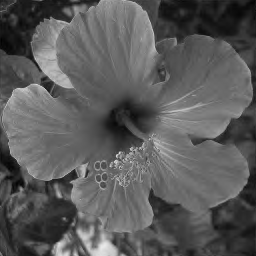
\includegraphics[width=.235\linewidth]{chapter-sampling/approx-8.png}&
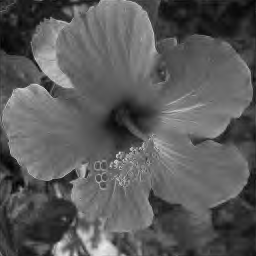
\includegraphics[width=.235\linewidth]{chapter-sampling/approx-16.png}\\
$f$&$M=N/4$&$M=N/8$&$M=N/16$
\end{tabular}
\caption{Best $M$-term wavelet approximations of a flower image with $N=256^2$ pixels. The orthonormal transform uses Daubechies wavelets with four vanishing moments, five levels, and periodic boundary conditions. Display intensities are clipped to $[0,1]$.}\label{fig-approx}
\end{figure}

The reconstruction $x\mapsto\Psi x$ is linear, but selecting the largest coefficients depends on the data. The approximation $f\mapsto\Psi x^\star$ is therefore nonlinear. For many piecewise smooth signals, wavelets give small errors with relatively few coefficients; the regularity of the signal controls the decay of this error~\cite[Chapter 9]{mallat2009a-wav}. Textures and fine oscillations can require substantially more terms.

The fraction $M/N$ counts retained coefficients; it is not a bit rate. A complete compressor must also quantize the retained values, describe their locations, and encode the resulting symbols. Entropy coding, introduced in the chapter on information theory, completes this step. Wavelet transforms also admit fast algorithms whose cost is proportional to the number of samples~\cite[Chapter 7]{mallat2009a-wav}.

\section{Inverse problems and regularization}
\label{sec-pb-inv}
\subsection{The observation model}
An inverse problem asks us to recover an unknown signal $f\in\RR^Q$ from measurements
\begin{equation}\label{eq-fwd-model}
 y=\Phi f+w\in\RR^P.
\end{equation}
The known linear operator $\Phi\in\RR^{P\times Q}$ describes acquisition, and $w$ represents unknown errors. Usually one applies $\Phi$ by an algorithm rather than storing this potentially enormous matrix.

\begin{figure}[htbp]\centering
\begin{tabular}{@{}c@{\hspace{3mm}}c@{\hspace{3mm}}c@{}}
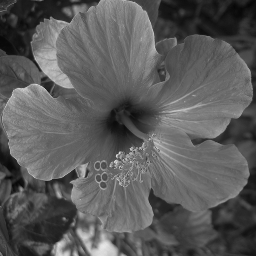
\includegraphics[width=.30\linewidth]{chapter-sampling/original.png}&
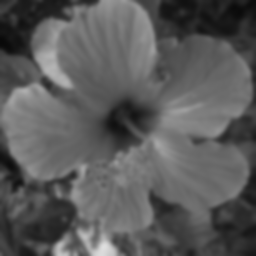
\includegraphics[width=.30\linewidth]{chapter-sampling/blurred.png}&
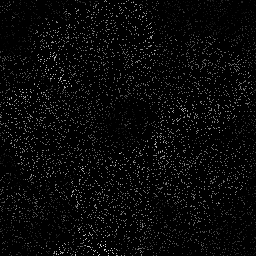
\includegraphics[width=.30\linewidth]{chapter-sampling/masked.png}\\
$f$&$\Phi f$: blur&$\Phi f$: mask
\end{tabular}
\caption{Two noiseless observation operators applied to the same flower image: Gaussian blurring and a mask retaining about $10\%$ of the pixels. Missing entries are displayed in black.}\label{fig-exemple-ip}
\end{figure}

Several standard problems fit this model:
\begin{itemize}
\item Denoising: $\Phi=\mathrm{Id}$ and $P=Q$.
\item Deblurring: $\Phi f=\phi\star f$, with a filter $\phi$ describing the blur and a specified boundary convention.
\item Missing data: $\Phi$ selects observed coordinates. Equivalently, one may keep the full array and use the diagonal mask $\Phi=\operatorname{diag}(\mu_q)$, where $\mu_q\in\{0,1\}$.
\item Tomography: $\Phi$ models line integrals of the object, as in a discretized Radon transform.
\end{itemize}
If $\Phi$ has a nontrivial kernel, the measurements alone do not determine $f$. Even when a square $\Phi$ is invertible, its small singular values can amplify errors in $\Phi^{-1}y=f+\Phi^{-1}w$. Regularization introduces additional information to select a useful, stable reconstruction.

\subsection{Sparse regularization}
Assuming $f\approx\Psi x$ with few active coefficients leads to
\begin{equation}\label{eq-pbm-l0}
 x^\star\in\arg\min_{\norm{x}_0\le M}\norm{y-\Phi\Psi x}_2^2,
 \qquad f^\star=\Psi x^\star.
\end{equation}
For denoising in an orthonormal basis, this is hard thresholding of the coefficients of the \emph{observed signal $y$}. It gives the best sparse fit to $y$ for the chosen budget; it does not by itself guarantee the smallest error relative to the unknown clean signal $f$. For a general acquisition operator, $\Phi\Psi$ is not orthogonal, and the simple thresholding formula no longer solves the problem.

Greedy algorithms and convex relaxation provide two ways to approach this difficulty~\cite{MallatMP,2014-vaiter-ps-review}. To motivate convex relaxation, consider
\[
 \norm{x}_\alpha^\alpha=\sum_{n=1}^N|x_n|^\alpha,\qquad \alpha>0.
\]
For each fixed vector $x$, this quantity tends to $\norm{x}_0$ as $\alpha\downarrow0$. The sets $B_\alpha=\{x:\sum_n|x_n|^\alpha\le1\}$ lie in $[-1,1]^N$ and converge, in Hausdorff distance, to
\[
 B_0=\{x\in[-1,1]^N:\norm{x}_0\le1\}.
\]
This limiting set consists of the coordinate-axis segments, including the origin. The set $\{x:\norm{x}_0\le1\}$ without the box restriction instead contains the entire, unbounded coordinate axes.

\begin{figure}[htbp]\centering
\begin{tabular}{@{}c@{\hspace{2mm}}c@{\hspace{2mm}}c@{\hspace{2mm}}c@{\hspace{2mm}}c@{}}
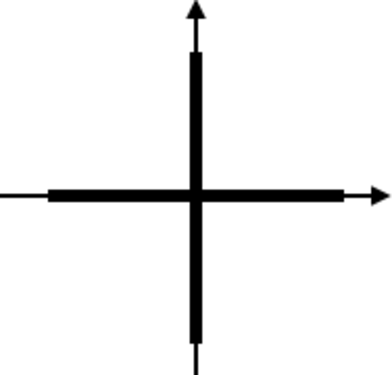
\includegraphics[width=.185\linewidth]{balls/l0}&
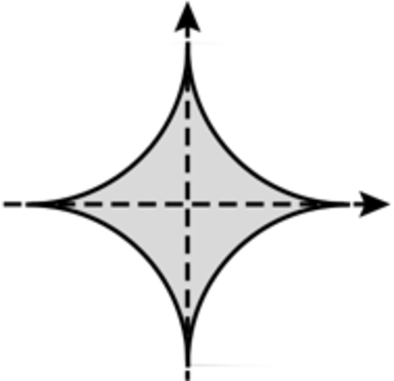
\includegraphics[width=.185\linewidth]{balls/l12}&
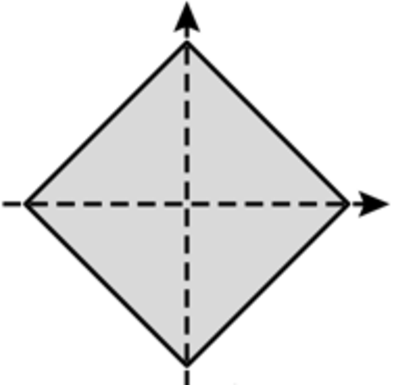
\includegraphics[width=.185\linewidth]{balls/l1}&
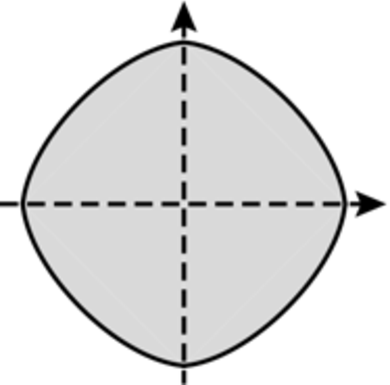
\includegraphics[width=.185\linewidth]{balls/l32}&
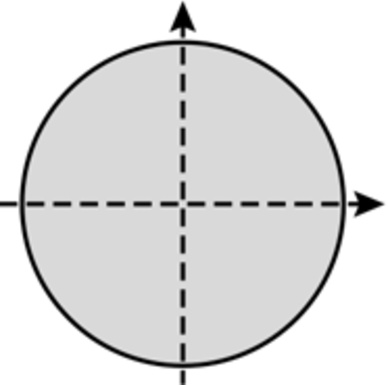
\includegraphics[width=.185\linewidth]{balls/l2}\\
$\alpha=0$&$\alpha=1/2$&$\alpha=1$&$\alpha=3/2$&$\alpha=2$
\end{tabular}
\caption{The sets $B_\alpha$ in two dimensions. The first panel shows the bounded limiting set $B_0$.}\label{fig-boules}
\end{figure}

Within this family, $\norm{\cdot}_\alpha$ is a norm and $B_\alpha$ is convex precisely when $\alpha\ge1$. The choice $\alpha=1$ balances convexity with a geometry that favors zero coefficients. This leads to the constrained Lasso problem
\begin{equation}\label{eq-pbm-l1}
 x^\star\in\arg\min_{\norm{x}_1\le\tau}\frac12\norm{Ax-y}_2^2,
 \qquad A=\Phi\Psi.
\end{equation}
Increasing $\tau$ allows a closer fit to the measurements, but can also fit their errors. The parameter must be chosen with the noise level, operator, and signal model in mind. Sending $\tau$ to infinity removes the regularization and generally leaves many possible reconstructions when $P<N$.

Two closely related formulations are useful:
\begin{align}
 &\min_x\ \frac12\norm{Ax-y}_2^2+\lambda\norm{x}_1,
 &&\lambda>0,\label{eq-lasso-penalized}\\
 &\min_x\ \norm{x}_1\quad\text{subject to }\norm{Ax-y}_2\le\varepsilon,
 &&\varepsilon\ge0.\label{eq-bpdn}
\end{align}
The penalized formulation trades data fit against sparsity. The second formulation, basis pursuit denoising, is convenient when an error bound $\varepsilon$ is known. For $\varepsilon=0$, it becomes basis pursuit, $\min_{Ax=y}\norm{x}_1$. These formulations are connected through suitable Lagrange multipliers; their parameters are not interchangeable numerical values. Early developments include seismic inversion, basis pursuit, and the Lasso~\cite{santosa1986linear,chen1999atomi,tibshirani1996regre}.

\begin{figure}[htbp]\centering
\begin{tabular}{@{}c@{\hspace{3mm}}c@{\hspace{3mm}}c@{}}
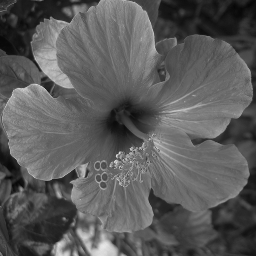
\includegraphics[width=.30\linewidth]{chapter-sampling/original.png}&
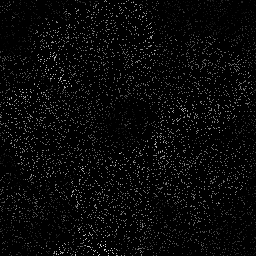
\includegraphics[width=.30\linewidth]{chapter-sampling/masked.png}&
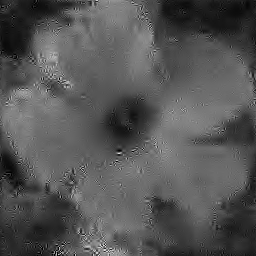
\includegraphics[width=.30\linewidth]{chapter-sampling/reconstructed.png}\\
$f$&$y$&$f^\star=\Psi x^\star$
\end{tabular}
\caption{Reconstruction from 6,554 observed pixels out of $256^2$ (about $10\%$). The penalized problem~\eqref{eq-lasso-penalized} is solved numerically with $\lambda=0.005$, intensities in $[0,1]$, and the same orthonormal wavelets as in Figure~\ref{fig-approx}. The remaining texture errors illustrate the limits of the model.}\label{fig-inpainting}
\end{figure}

Convexity makes global optimization possible, but the large dimension and the nondifferentiability of $\norm{x}_1$ still require suitable algorithms. Proximal methods exploit the explicit soft-thresholding operation associated with this penalty~\cite{combettes2011proximal}. A numerical solver reaches a prescribed accuracy, rather than an exact real-valued solution after a guaranteed small number of operations.

\subsection{Why the geometry matters}
In two dimensions, an $\ell^1$ ball has corners on the coordinate axes. A level set of the data-fitting term can first meet the ball at one of these corners, producing a zero coefficient. The round $\ell^2$ ball typically gives two nonzero coefficients in the same configuration (Figure~\ref{fig-l1-vs-l2}). This is an explanation of a tendency, not a guarantee for every operator or every datum: a contact along a face can give several minimizers, and an $\ell^1$ solution need not be sparse enough to recover the truth.

\begin{figure}[htbp]\centering
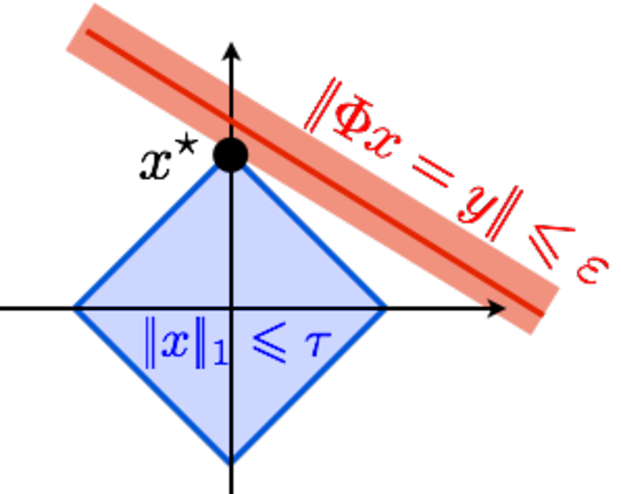
\includegraphics[width=.36\linewidth]{l1-vs-l2/l1}\hspace{8mm}
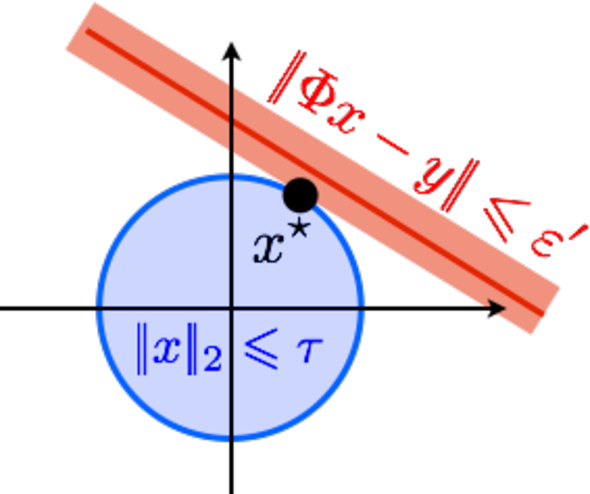
\includegraphics[width=.36\linewidth]{l1-vs-l2/l2}
\caption{Constrained data fitting with an $\ell^1$ ball (left) and an $\ell^2$ ball (right). Starting from $\varepsilon=0$, enlarge the strip $\{x:\norm{Ax-y}_2\le\varepsilon\}$ until it first meets the constraint ball. The contact point minimizes the residual over that ball.}\label{fig-l1-vs-l2}
\end{figure}

Recovery depends on how the measurement operator acts on sparse vectors. Increasing the ambient dimension alone does not improve it. Precise conditions are available for many random and structured operators; convolution and Fourier acquisition require assumptions adapted to their geometry~\cite{candes-towards2013,2015-duval-focm,AdcockBreaking,Chauffert14}.

\section{Compressed sensing}
\subsection{Measuring combinations of pixels}
Conventional transform coding first acquires $Q$ samples and then keeps a much smaller representation. Compressed sensing asks whether we can instead acquire $P\ll Q$ carefully chosen linear measurements and reconstruct a signal that is sparse, or approximately sparse, in a known basis.

The single-pixel camera developed at Rice University illustrates this idea~\cite{DuarteSinglePixel}. A grid of $Q$ micromirrors directs selected portions of the light towards one detector; other mirrors direct light away from it. For each pattern $p$, the detector measures the sum
\[
 y_p=\sum_{q=1}^Q\Phi_{p,q}\int_{c_q}\tilde f(s)\,\d s+w_p
     =\sum_{q=1}^Q\Phi_{p,q}f_q+w_p,
 \qquad \Phi_{p,q}\in\{0,1\}.
\]
The mirrors do not record individual pixels. Changing their configuration produces the vector $y\in\RR^P$ directly. The scene must remain sufficiently stable during these measurements. Complementary patterns, or a calibrated measurement of total light, can convert $0/1$ measurements into centered signed measurements.

\begin{figure}[htbp]\centering
\begin{tabular}{@{}c@{\hspace{2mm}}c@{\hspace{2mm}}c@{}}
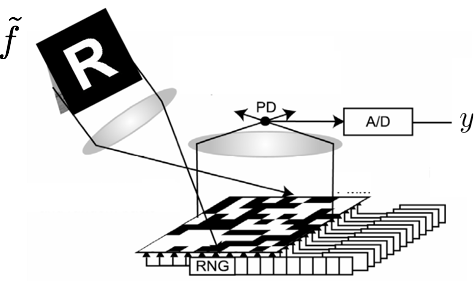
\includegraphics[width=.45\linewidth]{single-pixel/single-pixel-schema}&
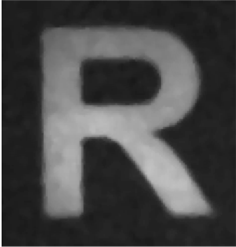
\includegraphics[width=.24\linewidth]{single-pixel/reconstruction-1}&
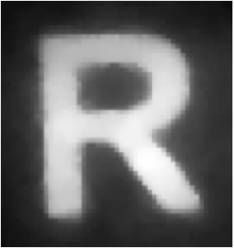
\includegraphics[width=.24\linewidth]{single-pixel/reconstruction-6}\\
Acquisition&$f$&$f^\star$
\end{tabular}
\caption{Single-pixel acquisition and the original reconstruction example, reproduced from the material accompanying~\cite{DuarteSinglePixel}. The stated measurement reduction factor is $Q/P=6$, so that $P/Q\approx1/6$.}\label{fig-single-pixel}
\end{figure}

\subsection{A recovery guarantee}
Here is a standard form of the compressed-sensing guarantee~\cite{candes2006stable,donoho2006compressed}. Suppose $\Psi$ is an orthonormal basis of $\RR^N$, $f=\Psi x_0$, and $A=\Phi\Psi$ has independent Gaussian entries with mean zero and variance $1/P$. Equivalently, $\Phi$ may be chosen with that Gaussian distribution, since it is invariant under multiplication by a fixed orthogonal matrix.

There are universal positive constants $C,c,C_0,C_1$ such that, for $1\le M\le N$ and
\begin{equation}\label{eq-cs-contrainte}
 P\ge C M\log(eN/M),
\end{equation}
with probability at least $1-2e^{-cP}$ over the choice of $A$, the following bound holds simultaneously for all $x_0$ and all errors with $\norm{w}_2\le\varepsilon$. Any solution $x^\star$ of~\eqref{eq-bpdn}, with $y=Ax_0+w$, satisfies
\begin{equation}\label{eq-cs-error}
 \norm{x^\star-x_0}_2
 \le C_0\frac{\sigma_M(x_0)_1}{\sqrt M}+C_1\varepsilon,
 \qquad
 \sigma_M(x_0)_1=\min_{\norm{z}_0\le M}\norm{x_0-z}_1.
\end{equation}
The logarithm in~\eqref{eq-cs-contrainte} is natural; changing its base only changes the constant. The interesting compressed regime is one in which the required $P$ is smaller than $N$.

The quantity $\sigma_M(x_0)_1$ is the sum of the magnitudes of the discarded coefficients after keeping the $M$ largest. If $x_0$ is exactly $M$-sparse and the noiseless problem uses $\varepsilon=0$ (hence $w=0$), both terms in~\eqref{eq-cs-error} vanish: basis pursuit recovers $x_0$ exactly. For approximately sparse signals and noisy measurements, the two terms separate the approximation error from the measurement error. Orthonormality gives the same Euclidean error for the reconstructed signal, $\norm{\Psi x^\star-f}_2=\norm{x^\star-x_0}_2$.

One route to this theorem is the restricted isometry property: $A$ approximately preserves Euclidean lengths of vectors supported on sufficiently small sets. Random matrices satisfy this property when the number of measurements has the order in~\eqref{eq-cs-contrainte}. Appropriate centered subgaussian designs also admit guarantees, with constants depending on their distribution. A raw $0/1$ sensing matrix requires the centering and normalization to be accounted for; it is not the Gaussian model stated above.

The theorem concerns a number of real measurements, not a number of bits. Their precision, quantization, and storage must still be considered. The sensing matrix must be known to the reconstruction algorithm, for instance through a shared random seed. Keeping that matrix secret is not, by itself, a cryptographic security guarantee. Likewise, savings in acquisition time or energy depend on the physical apparatus and the reconstruction cost.

Structured acquisition, including magnetic resonance imaging, imposes additional constraints: one cannot generally choose arbitrary independent Gaussian measurements. Sampling trajectories and sparsity models must therefore be analyzed together~\cite{AdcockBreaking,Chauffert14}. The guiding principle remains to design acquisition and reconstruction jointly, using a model that reflects the data.

\paragraph*{Further reading.}
The interplay between approximation, inverse problems, and optimization extends beyond sparsity. Other penalties encode smoothness, low rank, or geometric structure. The review~\cite{2014-vaiter-ps-review} develops these ideas, and the Numerical Tours~\cite{2011-peyre-cise} provide computational examples.

\ifdefined\StandaloneChapter
\paragraph*{Acknowledgements.}
I thank Charles Dossal, Jalal Fadili, Samuel Vaiter, Stéphane Seuret, and the anonymous reviewer of the original text for their help.
\fi
